%%=============================================================================
%% Literatuurstudie
%%=============================================================================

\chapter{\IfLanguageName{dutch}{Literatuurstudie}{State of the art}}%
\label{ch:literatuurstudie}

% Tip: Begin elk hoofdstuk met een paragraaf inleiding die beschrijft hoe
% dit hoofdstuk past binnen het geheel van de bachelorproef. Geef in het
% bijzonder aan wat de link is met het vorige en volgende hoofdstuk.

% Pas na deze inleidende paragraaf komt de eerste sectiehoofding.

% Dit hoofdstuk bevat je literatuurstudie. De inhoud gaat verder op de inleiding, maar zal het onderwerp van de bachelorproef *diepgaand* uitspitten. De bedoeling is dat de lezer na lezing van dit hoofdstuk helemaal op de hoogte is van de huidige stand van zaken (state-of-the-art) in het onderzoeksdomein. Iemand die niet vertrouwd is met het onderwerp, weet nu voldoende om de rest van het verhaal te kunnen volgen, zonder dat die er nog andere informatie moet over opzoeken \autocite{Pollefliet2011}.

% Je verwijst bij elke bewering die je doet, vakterm die je introduceert, enz.\ naar je bronnen. In \LaTeX{} kan dat met het commando \texttt{$\backslash${textcite\{\}}} of \texttt{$\backslash${autocite\{\}}}. Als argument van het commando geef je de ``sleutel'' van een ``record'' in een bibliografische databank in het Bib\LaTeX{}-formaat (een tekstbestand). Als je expliciet naar de auteur verwijst in de zin (narratieve referentie), gebruik je \texttt{$\backslash${}textcite\{\}}. Soms is de auteursnaam niet expliciet een onderdeel van de zin, dan gebruik je \texttt{$\backslash${}autocite\{\}} (referentie tussen haakjes). Dit gebruik je bv.~bij een citaat, of om in het bijschrift van een overgenomen afbeelding, broncode, tabel, enz. te verwijzen naar de bron. In de volgende paragraaf een voorbeeld van elk.

% \textcite{Knuth1998} schreef een van de standaardwerken over sorteer- en zoekalgoritmen. Experten zijn het erover eens dat cloud computing een interessante opportuniteit vormen, zowel voor gebruikers als voor dienstverleners op vlak van informatietechnologie~\autocite{Creeger2009}.

% Let er ook op: het \texttt{cite}-commando voor de punt, dus binnen de zin. Je verwijst meteen naar een bron in de eerste zin die erop gebaseerd is, dus niet pas op het einde van een paragraaf.

% \begin{figure}
%   \centering
%   
\includegraphics[width=0.8\textwidth]{grail.jpg}
%   \caption[Voorbeeld figuur.]{\label{fig:grail}Voorbeeld van invoegen van een figuur. Zorg altijd voor een uitgebreid bijschrift dat de figuur volledig beschrijft zonder in de tekst te moeten gaan zoeken. Vergeet ook je bronvermelding niet!}
% \end{figure}

% \begin{listing}
%   \begin{minted}{python}
%     import pandas as pd
%     import seaborn as sns

%     penguins = sns.load_dataset('penguins')
%     sns.relplot(data=penguins, x="flipper_length_mm", y="bill_length_mm", hue="species")
%   \end{minted}
%   \caption[Voorbeeld codefragment]{Voorbeeld van het invoegen van een codefragment.}
% \end{listing}

% \lipsum[7-20]

% \begin{table}
%   \centering
%   \begin{tabular}{lcr}
%     \toprule
%     \textbf{Kolom 1} & \textbf{Kolom 2} & \textbf{Kolom 3} \\
%     $\alpha$         & $\beta$          & $\gamma$         \\
%     \midrule
%     A                & 10.230           & a                \\
%     B                & 45.678           & b                \\
%     C                & 99.987           & c                \\
%     \bottomrule
%   \end{tabular}
%   \caption[Voorbeeld tabel]{\label{tab:example}Voorbeeld van een tabel.}
% \end{table}

Dit hoofdstuk biedt de stand van zaken en theoretische onderbouwing voor de vakgebieden die aan bod komen tijdens de ontwikkeling van de \emph{Proof of Concept}.

\section{\emph{Unified Modeling Language} (\emph{UML})}%
\label{sec:uml}

``\emph{Unified Modeling Language}'', of afgekort \emph{UML}, is een taal/framework die binnen de softwareontwikkeling-discipline geaccepteerd is als de standaard voor het weergeven van object-georiënteerde modellen. \emph{UML} wordt hoofdzakelijk gebruikt in de industrie-, business- en IT-sector, met als doel om de ontwerp- en implementatiefase te ondersteunen met verscheidene diagrammen. Deze kunnen door zowel business als technische stakeholders geïnterpreteerd worden voor hun respectievelijke doeleinden. \autocite{Koc2021}

Binnen de opleiding \emph{Toegepaste Informatica} worden er momenteel voornamelijk twee \emph{UML}-modeling programma's gebruikt en aangeraden; \emph{Visual Paradigm} en \emph{draw.io}. Dit zijn twee tools die (onder andere) werden geëvalueerd tijdens een vergelijkende studie van \textcite{Lu2023}, waarin \emph{Visual Paradigm} 122/165 (tweede plaats) en \emph{draw.io} 114/165 (achtste plaats, maar nog boven het gemiddelde) scoorden. Deze score is gebaseerd op hoe goed deze tools de verschillende diagramtypen ondersteunen, alsook of deze al dan niet bepaalde functionaliteiten bevatten zoals bestandsexportering en collaboratie.

Deze \emph{UML}-modeling programma's zijn \emph{GUI}-gebaseerd, en werken dus eerder met een drag-en-drop systeem. Er bestaan echter ook alternatieve tools zoals \emph{PlantUML} en \emph{MermaidJS}\footnote{\url{https://mermaid.js.org}}, die niet doorgaans vanuit de opleiding worden aangereikt. Deze maken, in tegenstelling tot \emph{Visual Paradigm} en \emph{draw.io}, gebruik van declaratieve talen waarmee men \emph{UML}-diagrammen kan ontwerpen via menselijk leesbare tekstbestanden, wat ook gemakkelijker te onderhouden is met versiebeheertools zoals \emph{Git}\footnote{\url{https://git-scm.com/}} \autocite{Romeo2025}.
Deze tools zijn ook open-source; de broncode van deze software is voor iedereen beschikbaar, wat voor studenten en docenten binnen de opleiding bijzonder interessant is.

\subsection{Diagrammen}%

Volgens \textcite{Padmanabhan2012} worden binnen \emph{UML} er veertien diagramtypen onderscheiden volgens de volgende overkoepelende categoriëen; \emph{Structure}, \emph{Behavior} en \emph{Interaction Diagrams}. Hier zijn een aantal van deze diagramtypen die het meest binnen de opleiding \emph{Toegepaste Informatica} toegelicht worden:

\begin{description}
  \item \textbf{\emph{Use Case Diagram}}: Beschrijft welke actoren (gebruikers, externe systemen) met een gegeven systeem interageren en welke functionaliteit zij gebruiken. Dit diagram is nuttig om de scope en de rollen binnen dit systeem te verduidelijken.
  \item \textbf{\emph{Class Diagram}}: Toont de klassen in een systeem met hun attributen, methoden en relaties (associaties, erfenis, compositie). Deze diagrammen zijn typisch op softwarecode gericht.
  \item \textbf{\emph{Deployment Diagram} (of implementatiediagram)}: Richt zich op de (al dan niet virtuele) nodes (servers, containers, netwerkapparatuur) en de daarop gedeployde artefacten (\emph{packages}, \emph{services}). Dit diagram sluit nauw aan bij een netwerkdiagram zoals die in DevOps-scenario's voorkomen.
  \item \textbf{\emph{Activity Diagram}}: Beschrijft de flow van controle en gegevens in een proces. Dit kan toegepast worden op een deployment pipeline of een provisioning workflow in een \emph{Infrastructure-as-Code}-context.
  \item \textbf{\emph{Sequence Diagram}}: Legt vast welke berichten in welke volgorde uitgewisseld worden tussen objecten of componenten, bijvoorbeeld tussen een webserver en een databank tijdens een typische request-flow.
\end{description}

\subsection{\emph{PlantUML}}%

\emph{PlantUML} is een open-source tool waarmee \emph{UML}- en aanverwante diagrammen gegenereerd kunnen worden op basis van een declaratief en menselijk leesbaar tekstformaat \autocite{PlantUML2026}.

De tool ondersteunt een brede waaier aan diagramtypen, waaronder vele \emph{UML}-diagrammen (\emph{Class Diagrams}, \emph{Deployment Diagrams}, \emph{Activity Diagrams}, \ldots), maar dus ook notaties die niet strikt genomen onder \emph{UML} vallen zoals netwerkdiagrammen, mindmaps en \emph{GANTT}-schemas \autocite{PlantUML2025}.

\emph{PlantUML} kan op verschillende manieren gebruikt worden; via de online webinterface\footnote{https://www.plantuml.com/plantuml}, een lokale installatie of een \emph{Docker}-container. Er worden ook verscheidene integraties aangeboden zoals plugins voor gangbare \emph{IDE}'s (\emph{Visual Studio Code}, \emph{IntelliJ IDEA} en \emph{Eclipse}) en documentatie- en wiki-tools (\emph{Confluence} en \emph{Markdown}).

Aangezien de diagramdefinities gewone tekstbestanden zijn (met ``\texttt{.puml}'' als bestandsextensie), lenen ze zich goed tot versiebeheer met \emph{Git}. \autocite{PlantUML2025a}

Het volgende codefragment stelt een voorbeeld van een implementatiediagram voor, met vijf nodes en hun bijhorende connecties.

\begin{codeblock}
  \begin{lstlisting}[language=plantuml]
@startuml

node node1
node node2
node node3
node node4
node node5
node1 -- node2 : label1
node1 .. node3 : label2
node1 ~~ node4 : label3
node1 == node5

@enduml
\end{lstlisting}
  \caption[Voorbeeld implementatiediagram in tekstformaat (\emph{PlantUML})]{Tekstformaat voor een voorbeeld van een implementatiediagram, uitgedrukt in \emph{PlantUML} \autocite{PlantUML2025}.}
  \label{code:depdiag_vb_puml}
\end{codeblock}

\emph{PlantUML} verwerkt vervolgens deze tekst en genereert op basis hiervan de volgende afbeelding.

\begin{figure}[H]
  \centering
  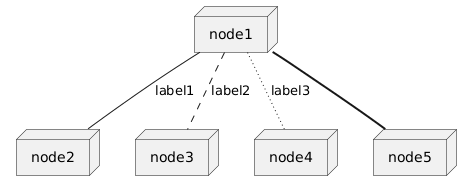
\includegraphics[width=0.5\textwidth]{../graphics/depdiag_vb_puml.png}
  \caption[Voorbeeld implementatiediagram in afbeeldingsformaat (\emph{PlantUML})]{Afbeeldingsformaat voor een voorbeeld van een implementatiediagram, gegenereerd door \emph{PlantUML}. \autocite{PlantUML2025}}
\end{figure}

\subsection{\emph{MermaidJS}}%

\emph{MermaidJS} is een gelijkaardige, open-source tool (gebaseerd op \emph{JavaScript}), die tekstuele, \emph{Markdown}-geïnspireerde syntax (met ``\texttt{.mermaid}'' als bestandsextensie) omzet naar diagrammen in afbeeldingsformaat.

Het wordt vaak gebruikt om documentatie in \emph{Markdown} (bijvoorbeeld in \emph{README}-bestanden op repositories) te verrijken met \emph{flowcharts}, \emph{Sequence Diagrams}, \emph{Class Diagrams} en \emph{GANTT}-schemas zonder een zware grafische editor te hoeven openen. \autocite{Mermaid2019}

Het volgende codefragment beschrijft een architectuurplan (vergelijkbaar met een netwerkdiagram), bestaande uit een server verbonden met een database, met elk hun bijhorende opslagmedia.

\begin{codeblock}
  \begin{lstlisting}
architecture-beta
    group api(cloud)[API]

    service db(database)[Database] in api
    service disk1(disk)[Storage] in api
    service disk2(disk)[Storage] in api
    service server(server)[Server] in api

    db:L -- R:server
    disk1:T -- B:server
    disk2:T -- B:db
\end{lstlisting}
  \caption[Eenvoudig infrastructuurdiagram in \emph{MermaidJS}]{Tekstformaat voor een voorbeeld van een architectuurplan, uitgedrukt in \emph{MermaidJS}. \autocite{Mermaid2026}}
  \label{code:archplan_vb_mermaid}
\end{codeblock}

\emph{MermaidJS} rendeert vervolgens op basis van deze code de volgende afbeelding.

\begin{figure}[H]
  \centering
  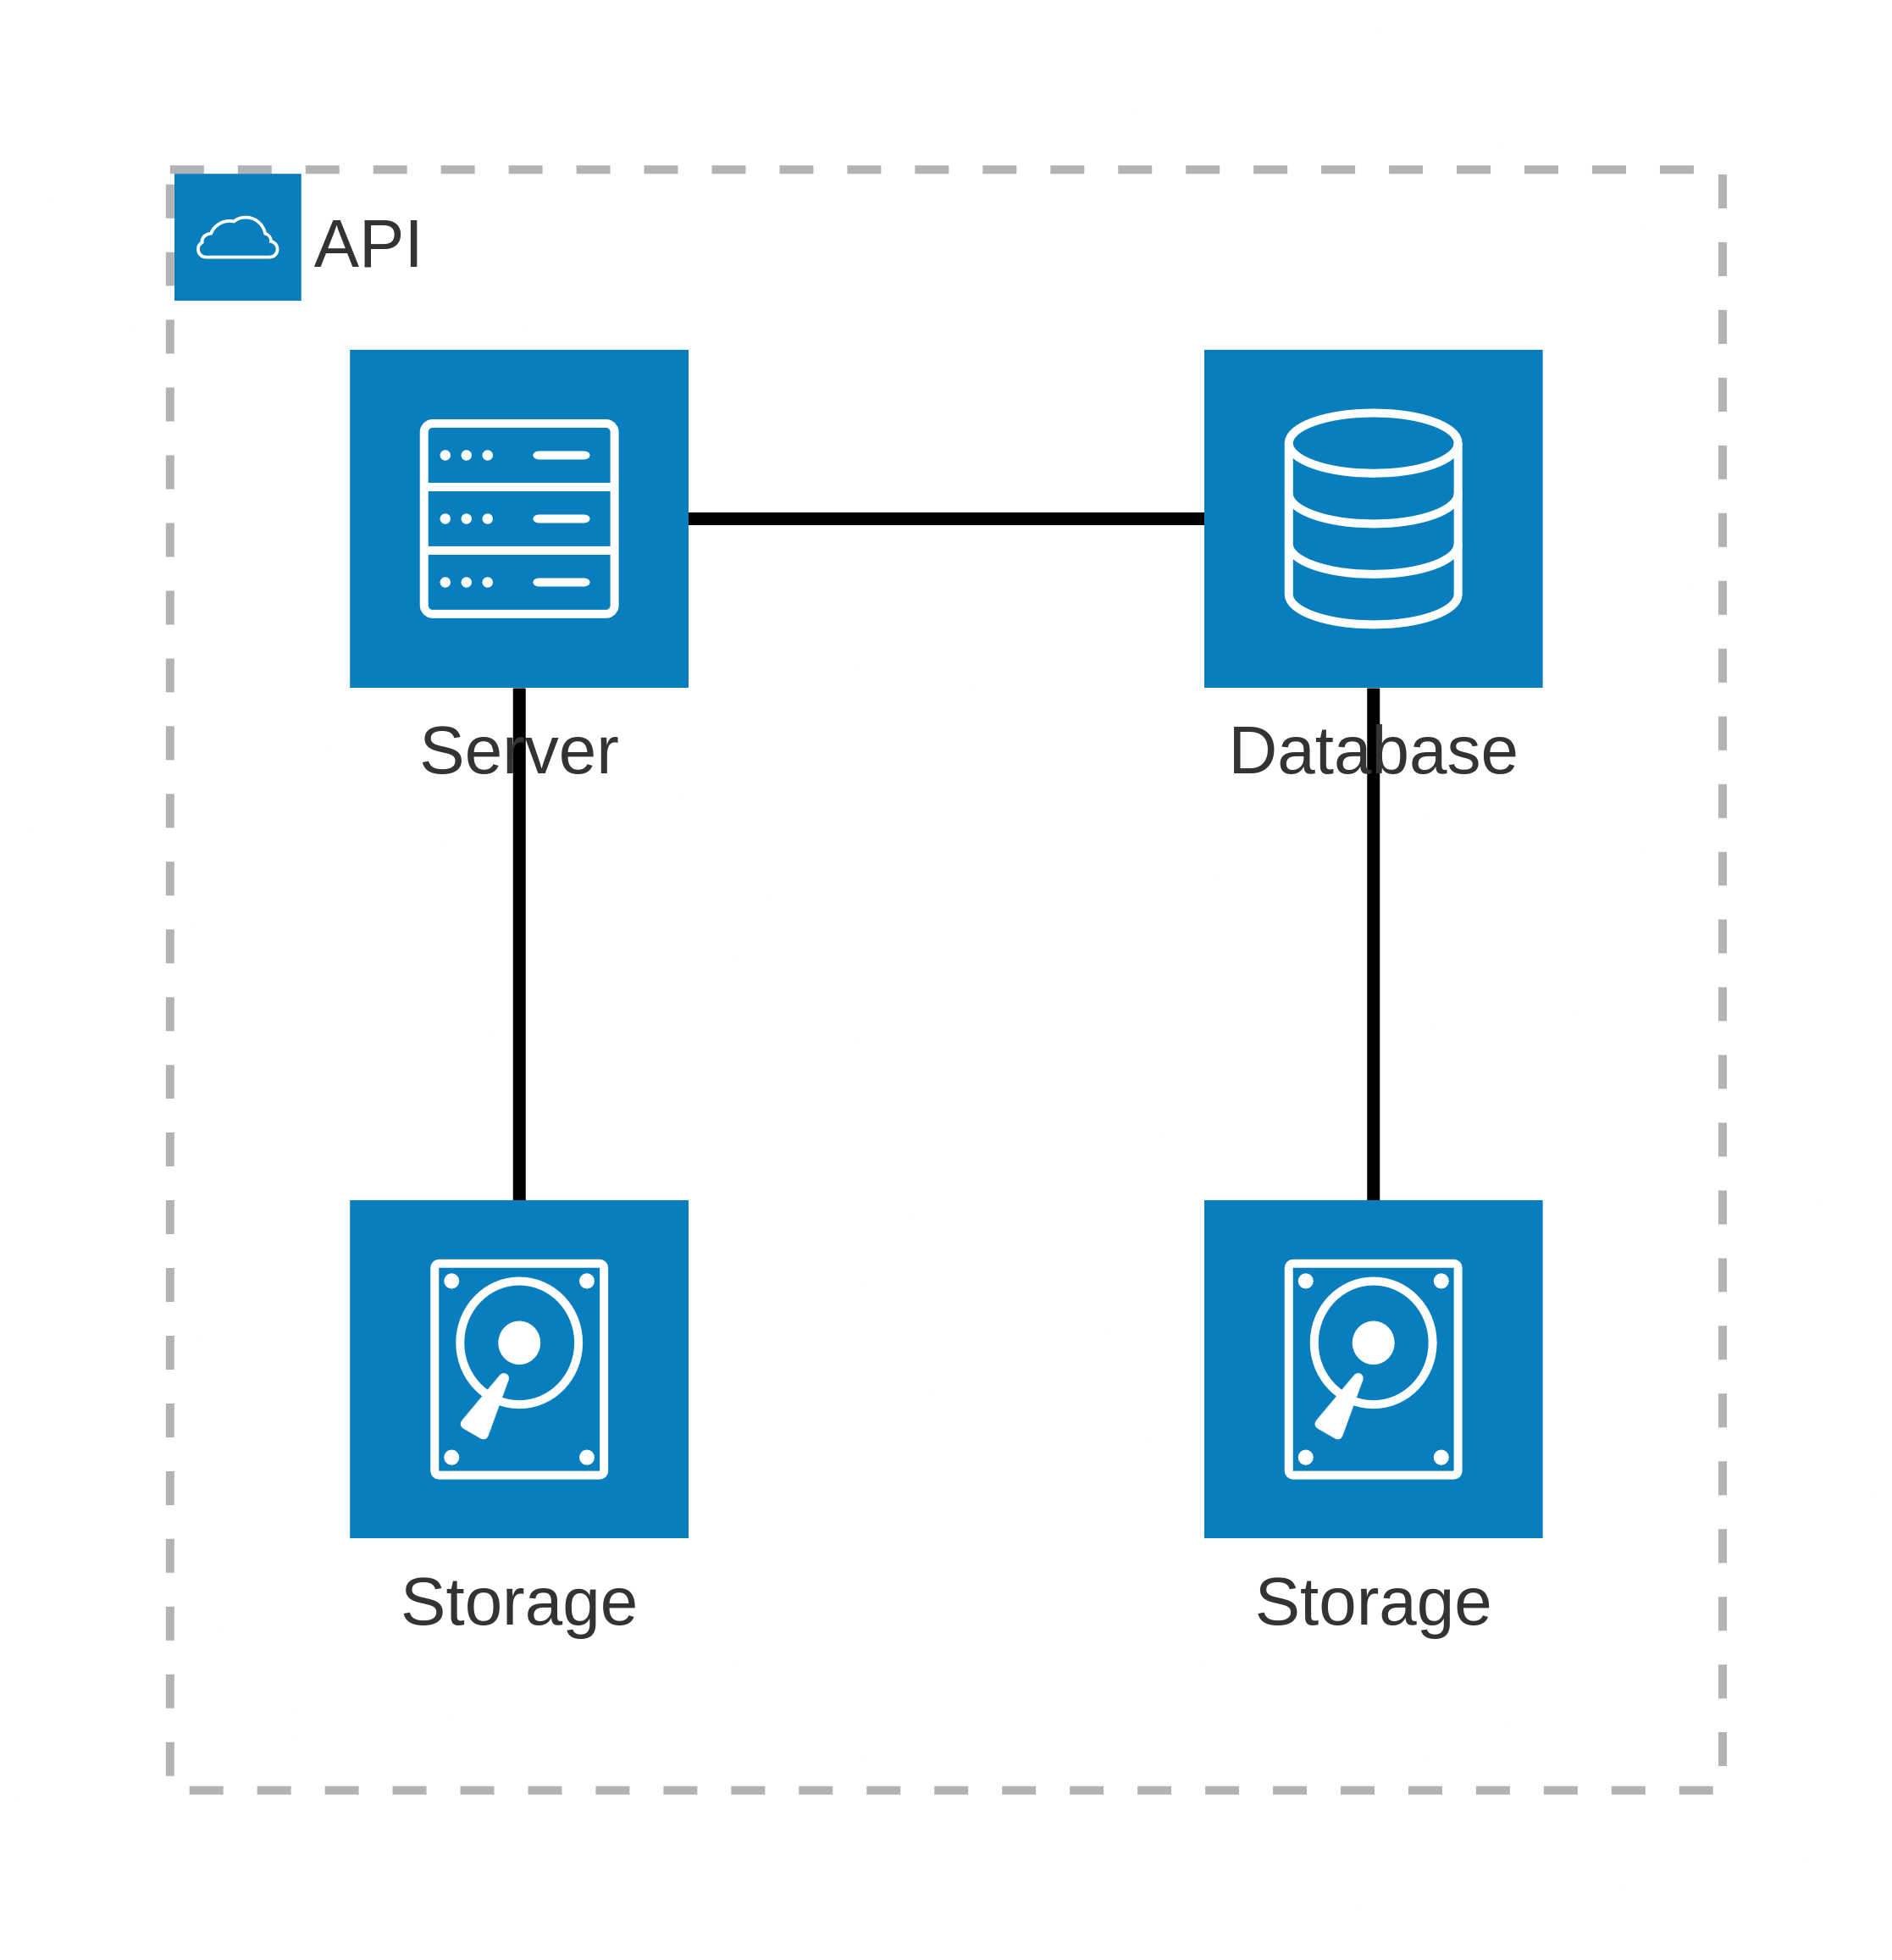
\includegraphics[width=0.5\textwidth]{../graphics/archplan_vb_mermaid.png}
  \caption[Voorbeeld architectuurplan in afbeeldingsformaat (\emph{MermaidJS})]{Afbeeldingsformaat voor een voorbeeld van een architectuurplan, uitgedrukt in \emph{MermaidJS} \autocite{Mermaid2026}.}
\end{figure}

\section{\emph{Infrastructure-as-Code}}%

\emph{Infrastructure-as-Code} (afgekort \emph{IaC}) is een praktijk binnen DevOps waarbij de nodes (fysiek of virtueel) binnen een IT-infrastructuur gedefinieerd en beheerd worden via machine-leesbare configuratiebestanden in plaats van via handmatige configuratie of grafische beheerconsoles \autocite{Rahman2019}.

Deze definities worden doorgaans onder versiebeheer geplaatst, waardoor men infrastructuurwijzigingen kan testen, herzien en eventueel terugdraaien zoals bij traditionele softwarecode.

De belangrijkste voordelen van \emph{IaC} zijn reproduceerbaarheid (omgevingen kunnen opnieuw identiek worden uitgerold), consistentie (vermindering van menselijke fouten en configuratiedrift), en een hogere snelheid van oplevering doordat de provisioning sterk geautomatiseerd wordt \autocite{Artac2017}.

\emph{IaC} staat echter niet in voor het configureren van nodes, dat is de taak van ``\emph{configuration management}''-tools zoals \emph{Ansible}, \emph{Puppet} en \emph{Chef}.

\textcite{Baer2025} onderscheidt grofweg twee benaderingen tot deze praktijk: een imperatieve stijl, waarin stap-voor-stap wordt beschreven welke acties er moeten worden uitgevoerd, en een declaratieve stijl, waarin enkel de gewenste eindsituatie van de infrastructuur wordt beschreven.
Moderne \emph{IaC}-tools zoals \emph{Terraform}, \emph{OpenTofu} en \emph{Vagrant} volgen hoofdzakelijk een declaratief model.

\subsection{\emph{Terraform}}%

\emph{Terraform} is een open-source ``\emph{Infrastructure-as-Code}'' tool van \emph{HashiCorp}, ontworpen om infrastructuur geautomatiseerd te provisioneren en te beheren over (meerdere) cloud- en on-premises platformen.
In plaats van infrastructuur handmatig aan te maken in een webconsole, definieert men de gewenste toestand in configuratiebestanden, waarna \emph{Terraform} aan de hand van verscheidene \emph{API}'s voor de betrokken platformen de nodige resources aanmaakt, wijzigt of verwijdert. \autocite{HashiCorp2024}

De configuraties worden geschreven in \emph{HashiCorp} Configuration Language (\emph{HCL}) (met ``\texttt{.tf}'' als bestandsextensie), een menselijk leesbare, declaratieve taal waarin men verschillende zaken kan definiëren zoals resources (zoals al dan niet virtuele nodes, maar ook bijvoorbeeld netwerken of \emph{DNS}-records), data sources (om externe data aan te reiken) en modules (sets van configuratiebestanden). \autocite{HashiCorp2025}

\emph{Terraform} ondersteunt honderden providers; dit varieert van providers ontwikkeld door officiële partners (zoals IBM en \emph{Ansible}) tot providers van third-party bedrijven (zoals \emph{Amazon AWS}, \emph{Microsoft Azure}, \emph{Google Cloud}, \ldots), wat het bijzonder flexibel maakt voor multi-cloud- en hybride omgevingen. \autocite{HashiCorp2025a}

Het volgende codefragment licht de structuur van \emph{HCL} toe via een eenvoudige topologie voor een \emph{AWS}-gebaseerde omgeving.

\begin{codeblock}
  \begin{minted}{terraform}
terraform {
  required_providers {
    aws = {
      source  = "hashicorp/aws"
      version = "~> 1.0.4"
    }
  }
}

variable "aws_region" {}

variable "base_cidr_block" {
  description = "A /16 CIDR range definition, such as 10.1.0.0/16, that the VPC will use"
  default = "10.1.0.0/16"
}
variable "availability_zones" {
  description = "A list of availability zones in which to create subnets"
  type = list(string)
}
provider "aws" {
  region = var.aws_region
}
resource "aws_vpc" "main" {
  # Referencing the base_cidr_block variable allows the network address
  # to be changed without modifying the configuration.
  cidr_block = var.base_cidr_block
}
resource "aws_subnet" "az" {
  # Create one subnet for each given availability zone.
  count = length(var.availability_zones)

  # For each subnet, use one of the specified availability zones.
  availability_zone = var.availability_zones[count.index]

  # By referencing the aws_vpc.main object, Terraform knows that the subnet
  # must be created only after the VPC is created.
  vpc_id = aws_vpc.main.id

  # Built-in functions and operators can be used for simple transformations of
  # values, such as computing a subnet address. Here we create a /20 prefix for
  # each subnet, using consecutive addresses for each availability zone,
  # such as 10.1.16.0/20 .
  cidr_block = cidrsubnet(aws_vpc.main.cidr_block, 4, count.index + 1 )
}
\end{minted}
  \caption[Voorbeeld \emph{Terraform}-configuratie]{Voorbeeld van een eenvoudige \emph{Terraform}-configuratie \autocite{HashiCorp2025}.}
  \label{code:terraform_vb}
\end{codeblock}

\subsection{\emph{OpenTofu}}%

\emph{OpenTofu} is een relatief recente speler, ontstaan als een community-gedreven fork van \emph{Terraform} in 2023. De drijfveer achter deze fork is de keuze van \emph{HashiCorp} om een licentiewijziging naar het \emph{Business Source License} (afgekort \emph{BSL}) voor \emph{Terraform} door te voeren. Dit bracht het bestuur in gevaar voor de bestaande community, die op lange termijn eerder leveranciersonafhankelijk willen blijven. \autocite{Gaddam2023}

Het project heeft als doel een volledig vrije, open-governance variant van de \emph{Terraform}-tooling te bieden, met langdurige compatibiliteit en transparante besluitvorming in de open-source gemeenschap.

Op technisch vlak positioneert \emph{OpenTofu} zich als een drop-in replacement voor \emph{Terraform 1.6.x} (en voorafgaande versies); bestaande configuraties in \emph{HCL} en de bekende \emph{CLI}-commando's blijven bruikbaar, zodat organisaties en projecten relatief eenvoudig kunnen migreren zonder hun codebase volledig te moeten herschrijven.
De tool ondersteunt dus dezelfde concepten (providers, resources, modules en state-bestanden) en streeft naar \emph{backwards compatibility}, terwijl op termijn nieuwe functionaliteit kan worden geïntroduceerd die niet noodzakelijk in \emph{Terraform} beschikbaar is. \autocite{OpenTofu2026}

\subsection{\emph{Vagrant}}%

\emph{Vagrant} is een tool van \emph{HashiCorp} voor het bouwen en beheren van (lokale) virtuele omgevingen via een tekstueel configuratiebestand (``\texttt{Vagrantfile}'').
Het doel van \emph{Vagrant} is om reproduceerbare ontwikkel- en testomgevingen te creëren die met één commando kunnen opgestart, geprovisioneerd en opnieuw vernietigd worden. \autocite{HashiCorp2026}

In de ``\texttt{Vagrantfile}'' specificeert men voor elke virtuele machine, onder andere, de base box (of het gastbesturingssysteem zoals \emph{AlmaLinux}, Alpine Linux, Ubuntu), het aantal \emph{CPU} cores, hoeveelheid werkgeheugen, welke netwerkconfiguratie van toepassing is, en welke provisioning-stappen moeten worden uitgevoerd.
Standaard ondersteunt \emph{Vagrant} providers zoals \emph{VirtualBox}, \emph{Hyper-V} en \emph{Docker}, maar via plugins kunnen ook andere platformen worden aangestuurd, waaronder \emph{VMware} of publieke cloudproviders. \autocite{HashiCorp2026a}

Voor provisioning kan \emph{Vagrant} gebruik maken van verschillende methodes zoals \emph{Bash}-scripts maar ook ``\emph{configuration management}''-tools (\emph{Ansible}/\emph{Chef}/\emph{Puppet}).
Dit maakt het mogelijk om via het ``\texttt{vagrant up}''-commando zowel de virtuele infrastructuur (via \emph{Vagrant}) als de configuratie van het gastbesturingssysteem (bijvoorbeeld via \emph{Ansible}-\emph{playbooks}) te automatiseren. \autocite{HashiCorp2026a}

Binnen de opleiding \emph{Toegepaste Informatica} wordt \emph{Vagrant} ingezet om snel identieke virtuele omgevingen uit te rollen waarin \emph{Ansible} de verdere configuratie en deployment van software verzorgt.

Het volgende codefragment licht een mogelijke, eenvoudige ``\texttt{Vagrantfile}'' toe.

\begin{codeblock}
  \begin{minted}{ruby}
Vagrant.configure("2") do |config|
  config.vm.box = "hashicorp-education/ubuntu-24-04"
  config.vm.box_version = "0.1.0"
  # Install Docker and dependencies
  config.vm.provision "shell", name: "install-dependencies", path: "install-dependencies.sh"
  # Start Terramino (can be rerun with vagrant provision --provision-with start-terramino)
  config.vm.provision "shell", name: "start-terramino", inline: <<-SHELL
    cd /home/vagrant/terramino-go
    docker compose up -d
  SHELL
  # Restart Terramino (can be rerun with vagrant provision --provision-with restart-terramino)
  # For quick changes that doesn't require rebuilding (e.g. frontend changes)
  config.vm.provision "shell", name: "restart-terramino", run: "never", inline: <<-SHELL
    docker compose restart
  SHELL
  # Reload Terramino (can be rerun with vagrant provision --provision-with reload-terramino)
  # For changes that require rebuilding (e.g. backend changes)
  config.vm.provision "shell", name: "reload-terramino", run: "never", inline: <<-SHELL
    /usr/local/bin/reload-terramino
  SHELL
end
\end{minted}
  \caption[Voorbeeld ``\texttt{Vagrantfile}'']{Voorbeeld van een eenvoudige ``\texttt{Vagrantfile}'' \autocite{HashiCorp2024a}.}
  \label{code:vagrantfile_vb}
\end{codeblock}

\section{\emph{Configuration management}}%

\emph{Configuration management} is het principe om een (grote) set van manuele, repetitieve configuratietaken (installeren van \emph{packages}, beheren van \emph{firewalls}, instellen van de default gateways en \emph{DNS}-servers, \ldots) automatisch te laten uitvoeren op servers. In het beste geval verloopt dit proces op een idempotente manier; op basis van dezelfde stappen wordt hetzelfde resultaat opgeleverd zonder afwijkingen, en vertoont het proces dus consistent gedrag. Deze manier van werken, analoog met het principe van \emph{Infrastructure-as-Code}, schaalt beter voor omgevingen met honderden of duizenden nodes, aangezien het aanzienlijk minder tijdrovend en vatbaar voor menselijke fouten is. \autocite{Likitha2022}

Als \emph{Infrastructure-as-Code} een omgeving automatisch opzet, staat \emph{configuration management} met andere woorden in voor het configuratie-aspect.

\emph{Ansible}, \emph{Puppet} en \emph{Chef} zijn drie open-source tools die in de praktijk het meest gebruikt worden om \emph{configuration management} toe te passen \autocite{Masek2018}.

\subsection{\emph{Ansible}}%

\emph{Ansible} is een open-source ``\emph{configuration management}''-tool die werkt zonder permanente \emph{agents} op de doelhosts: standaard maakt het verbinding via \emph{SSH} om taken uit te voeren.
Beheerders beschrijven de gewenste configuratie in menselijk leesbare YAML-bestanden, zogenaamde \emph{playbooks}, die bestaan uit taken (\emph{tasks}) en herbruikbare rollen (\emph{roles}). \autocite{Ansible2025}

Taken maken gebruik van (ingebouwde) modules om verscheidene systeem-gerelateerde objecten te beheren, zoals \emph{packages}, \emph{services}, gebruikers, bestanden en \emph{firewall}-regels.
Hier is de kracht van \emph{Ansible} dat men deze taken op declaratieve wijze kan schrijven in plaats van imperatief; men beschrijft \emph{wat} het eindresultaat moet zijn, niet \emph{hoe} men daar moet geraken. \emph{Ansible} biedt hier dus ook de mogelijkheid om \emph{playbooks} zo idempotent mogelijk te schrijven; bij herhaalde uitvoeringen krijgt men steeds hetzelfde, verwachte eindresultaat. \autocite{Stoeckl2025}

Dankzij een \emph{inventory}-bestand kunnen de taken van een \emph{playbook} identiek uitgevoerd worden op groepen van meerdere hosts, wat \emph{Ansible} geschikt maakt voor het configureren van tientallen of honderden servers in één keer. \autocite{Ansible2025}

Onderstaand voorbeeld toont een beknopte \emph{Ansible}-\emph{playbook} die twee taken uitvoert: de webserver en databankserver updaten op alle hosts in de overeenkomende groepen (``\texttt{webservers}'' en ``\texttt{databases}'').

\begin{codeblock}
  \begin{minted}{yaml}
---
- name: Update web servers
  hosts: webservers
  remote_user: root

  tasks:
  - name: Ensure apache is at the latest version
    ansible.builtin.yum:
      name: httpd
      state: latest

  - name: Write the apache config file
    ansible.builtin.template:
      src: /srv/httpd.j2
      dest: /etc/httpd.conf

- name: Update db servers
  hosts: databases
  remote_user: root

  tasks:
  - name: Ensure postgresql is at the latest version
    ansible.builtin.yum:
      name: postgresql
      state: latest

  - name: Ensure that postgresql is started
    ansible.builtin.service:
      name: postgresql
      state: started
\end{minted}
  \caption[Voorbeeld \emph{Ansible}-\emph{playbook}]{Voorbeeld van een eenvoudige \emph{Ansible}-\emph{playbook} \autocite{Ansible2025a}.}
  \label{code:ansible_playbook_vb}
\end{codeblock}

Deze \emph{playbook} kan herhaaldelijk uitgevoerd worden en telkens hetzelfde resultaat opleveren, wat het potentieel van \emph{Ansible} qua idempotentie (zeker voor de ingebouwde modules) illustreert.

\subsection{\emph{Puppet}}%

\emph{Puppet} is een ``\emph{configuration management}''- tool die gebruikmaakt van een declaratieve domeinspecifieke taal (gebaseerd op \emph{Ruby}) om de gewenste toestand van systemen te beschrijven.
Beheerders definiëren resources (zoals \emph{packages}, files en \emph{services}) in \emph{manifests}; \emph{Puppet} vergelijkt vervolgens de actuele toestand van een host met deze gewenste toestand en brengt enkel de noodzakelijke wijzigingen aan. \autocite{Perforce2026a}

Typisch wordt \emph{Puppet} ingezet in een ``\emph{server-agent}''-architectuur: een centrale \emph{Puppet}-server compileert de \emph{manifests} tot een \emph{catalog} en deelt deze catalog uit aan \emph{Puppet}-\emph{\emph{agent}s} op de beheerde hosts.
De \emph{agent} past de catalog toe, corrigeert eventuele configuratiedrift en rapporteert zijn status terug aan de server, waardoor beheerders op grote schaal configuraties kunnen afdwingen en monitoren. \autocite{Perforce2026b}

Het volgende \emph{manifest} toont vereenvoudigd aan hoe een server geconfigureerd kan worden met \emph{Puppet}:

\begin{codeblock}
  \begin{minted}{ruby}
file { 'ntp.conf':
  path    => '/etc/ntp.conf',
  ensure  => file,
  content => template('ntp/ntp.conf'),
  owner   => 'root',
  mode    => '0644',
}

package { 'ntp':
  ensure => installed,
  before => File['ntp.conf'],
}

service { 'ntpd':
  ensure    => running,
  subscribe => File['ntp.conf'],
}
\end{minted}
  \caption[Eenvoudig \emph{Puppet}-\emph{manifest} voor een webserver]{\autocite{Perforce2026}}
  \label{code:puppetvb}
\end{codeblock}

Wanneer de \emph{agent} dit \emph{manifest} meerdere keren toepast, zal \emph{Puppet} enkel wijzigingen maken als de werkelijke toestand (bijvoorbeeld ontbrekende bestanden of een gestopte \emph{service}) afwijkt van de beschreven gewenste toestand.

\subsection{\emph{Chef}}%

\emph{Chef} is een ``\emph{configuration management}''-tool en automatiseringsplatform dat \emph{Infrastructuur-as-Code} benadert via \emph{Ruby}-gebaseerde code.
Configuratie wordt georganiseerd in \emph{cookbooks}, die één of meerdere \emph{recipes} bevatten; een \emph{recipe} beschrijft met behulp van resources (zoals ``\texttt{package}'', ``\texttt{file}'' en ``\texttt{service}'') de gewenste toestand van een node.  \autocite{ProgressSoftware2026}

In een typische opstelling communiceren \emph{Chef}-clients op de beheerde nodes met een centrale \emph{Chef}-server, die \emph{cookbooks}, policies en \emph{run lists} beheert.
Tijdens een \emph{run} vraagt de client zijn \emph{run list} op, convergeert het systeem naar de in de \emph{recipes} gedefinieerde toestand en rapporteert het resultaat terug, wat een idempotente, herhaalbare configuratieworkflow oplevert. \autocite{ProgressSoftware2026a}

Onderstaande vereenvoudigde \emph{recipe} installeert een \emph{Apache} webserver, kiest op willekeurige basis \emph{PHP} of \emph{Perl} als scriptingtaal, en installeert deze vervolgens.

\begin{codeblock}
  \begin{minted}{ruby}
package 'httpd' do
  action :install
end

ruby_block 'randomly_choose_language' do
  block do
    if Random.rand > 0.5
      node.run_state['scripting_language'] = 'php'
    else
      node.run_state['scripting_language'] = 'perl'
    end
  end
end

package 'scripting_language' do
  package_name lazy { node.run_state['scripting_language'] }
  action :install
end
\end{minted}
  \caption[Eenvoudige \emph{Chef}-\emph{recipe} voor een webserver]{\autocite{ProgressSoftware2025}}
  \label{code:chefvb}
\end{codeblock}

Bij elke \emph{Chef}-\emph{run} wordt deze \emph{recipe} opnieuw geëvalueerd; als ``\texttt{httpd}'' al geïnstalleerd is en de client overeenkomt met de gewenste toestand, zullen er geen wijzigingen meer worden doorgevoerd, in lijn met het idempotente karakter van \emph{configuration management}. Als bij de volgende \emph{run} een andere scriptingtaal wordt gekozen, dan zullen de wijzigingen op basis daarvan uitgevoerd worden (de deinstallatie van de oude scriptingtaal, gevolgd door installatie van de nieuwe scriptingtaal).

\section{De opleiding Toegepaste Informatica (\emph{HOGENT})}%
\label{sec:opleiding}

\emph{Toegepaste Informatica} is een professionele bacheloropleiding van drie jaar aan \emph{HOGENT}, aangeboden door het \emph{Departement IT \& Digitale Innovatie} \autocite{HOGENT2024}. In het derde jaar kiezen studenten een keuzeprofiel dat aansluit bij hun interesse; voor studenten met een interesse in serverinfrastructuur, netwerken en automatisering is dat het keuzeprofiel ``\emph{IT infrastructure engineer}''.

De volgende subsecties beschrijven achtereenvolgend het relevante keuzeprofiel (``\emph{IT infrastructure engineer}''), drie \emph{OLODs} (opleidingsonderdelen) die er binnen vallen en centraal staan in deze bachelorproef, de \emph{Ansible}-rollen en de \emph{Ansible Skeleton} van Bert Van Vreckem, en tot slot een algemeen overzicht van de voornaamste tools die binnen de \emph{OLODs} in dit keuzeprofiel worden ingezet.

\subsection{``IT infrastructure engineer'' (Keuzeprofiel)}%
\label{subsec:keuzeprofiel}

Binnen dit keuzeprofiel zijn er drie \emph{OLODs} die relevant zijn voor deze bachelorproef, omdat ze elk op hun manier het ontwerpen en/of implementeren van virtuele serverinfrastructuren centraal stellen:

\begin{itemize}
  \item ``\emph{Cybersecurity Advanced}'' \autocite{HOGENT2025}
  \item ``\emph{Infrastructure Automation}'' \autocite{HOGENT2025a}
  \item ``\emph{DevOps Project: Operations}'' \autocite{HOGENT2025b}
\end{itemize}

De twee eerstgenoemde \emph{OLODs} stellen hierbij een initiële labo-omgeving beschikbaar via de \emph{GitHub}-organisatie \emph{HoGentTIN} \autocite{HoGentTIN2025,HoGentTIN2025a}. In elk van deze \emph{OLODs} wordt een basisinfrastructuur aangeboden waarop studenten verder kunnen bouwen; hoe deze infrastructuur opgezet, geconfigureerd en gedocumenteerd wordt, is telkens een kerndoelstelling van het \emph{OLOD}.

\subsection{``\emph{Cybersecurity Advanced}'' (\emph{OLOD})}%
\label{subsec:cybersec_adv}

Het \emph{OLOD} ``\emph{Cybersecurity Advanced}'' introduceert het concept van ``\emph{blue-teaming}'' -- het verdedigen van een netwerk tegen aanvallen -- aan de hand van een reeks virtuele labo's die individueel worden uitgevoerd \autocite{HOGENT2025}. De labo's draaien telkens rond een basisomgeving met meerdere virtuele machines die elk een specifieke rol opnemen (\emph{DNS}-server, webserver, databankserver, \ldots).

Het gebruik van \emph{configuration management} of \emph{UML}-diagrammen is hierbij niet strikt noodzakelijk, maar het geeft de student een aanzienlijk voordeel: de labo-omgeving is zo overzichtelijker en kan (na het manueel uitvoeren van elk labo) snel opnieuw opgezet worden met de relevante aanpassingen. De initiële labo-omgeving wordt alvast voorgesteld met een netwerkdiagram ontworpen via \emph{PlantUML} \autocite{HoGentTIN2025}, wat studenten een rechtstreekse link biedt tussen het diagram en de effectieve omgeving.

\subsection{``\emph{Infrastructure Automation}'' (\emph{OLOD})}%
\label{subsec:infra_auto}

``\emph{Infrastructure Automation}'' is een \emph{OLOD} dat een reeks labo's bevat die verschillende tools introduceren voor het automatisch opzetten, configureren en monitoren van serveromgevingen, waaronder \emph{Ansible}, \emph{Jenkins}\footnote{\url{https://www.jenkins.io/}}, \emph{Prometheus}\footnote{\url{https://prometheus.io/}} en \emph{Kubernetes}\footnote{\url{https://kubernetes.io/}} \autocite{HOGENT2025a}. In tegenstelling tot ``\emph{Cybersecurity Advanced}'' is het gebruik van \emph{configuration management} hier een centrale leerdoelstelling: de labo's vereisen dat studenten \emph{Ansible} inzetten om de virtuele machines te configureren.

De labo-omgeving voor dit \emph{OLOD} is gebaseerd op de ``\emph{Ansible Skeleton}'' van \textcite{Vreckem2025}: een sjabloon voor \emph{Ansible}-projecten met een geïntegreerde \emph{Vagrant}-omgeving (zie \autoref{subsec:bertvv}). Deze structuur -- met mappen zoals ``\texttt{ansible/}'', ``\texttt{ansible/host\_vars/}'', ``\texttt{ansible/group\_vars/}'' en een centrale ``\texttt{site.yml}''-\emph{playbook} -- vormt ook de uitvoerstructuur van de \emph{converter} die in deze bachelorproef wordt ontwikkeld \autocite{HoGentTIN2025a}.

\subsection{``\emph{DevOps Project: Operations}'' (\emph{OLOD})}%
\label{subsec:devops_ops}

``\emph{DevOps Project: Operations}'' is een \emph{OLOD} dat het tweede luik vormt van een tweeledig groepsproject \autocite{HOGENT2025b}, het eerste luik zijnde ``\emph{Real-life Integrated Software Engineering}'' (\emph{RISE}) voor de studenten binnen het keuzetraject ``\emph{full stack developer}''.
Het doel van het ``\emph{operations}-team'' is om de backend van een webapplicatie (bijvoorbeeld een \emph{.NET}- of \emph{Android}-\emph{package}) -- ontwikkeld door een parallel ``\emph{development}-team'' -- te ondersteunen met een productie-waardige serverinfrastructuur. Deze omgeving moet volledig geautomatiseerd kunnen opgezet worden via \emph{Infrastructure-as-Code}- en \emph{configuration management}-tools.

In tegenstelling tot de twee vorige \emph{OLODs} is het gebruik van een netwerkdiagram hier verplicht: de onderliggende architectuur moet gevisualiseerd worden voor zowel technische als niet-technische stakeholders via \emph{UML}-modelleringssoftware. Dit \emph{OLOD} combineert daarmee twee aspecten die centraal staan in deze bachelorproef: het ontwerpen van een infrastructuur via (\emph{UML}-)diagrammen, en het automatisch uitrollen ervan via \emph{IaC} en \emph{configuration management}.

\subsection{\emph{Ansible}-rollen en \emph{Ansible Skeleton} van Bert Van Vreckem}%
\label{subsec:bertvv}

Een aantal centrale bouwstenen binnen de bovenstaande \emph{OLODs} -- en bij uitbreiding binnen de \emph{converter} ontwikkeld in deze bachelorproef -- zijn de \emph{Ansible}-rollen en \emph{Ansible Skeleton} van \textcite{Vreckem2025}.
De \emph{Ansible Skeleton} is een sjabloon voor \emph{Vagrant}- en \emph{Ansible}-projecten dat een vaste mappenstructuur, een vooraf geconfigureerde ``\texttt{Vagrantfile}'' en hulpscripts omvat. Deze ``\texttt{Vagrantfile}'' is zo ontworpen zodat men enkel in een apart ``\texttt{vagrant-hosts.yml}''-bestand hosts moet definiëren om deze vervolgens eenvoudig op te starten met het ``\texttt{vagrant up}''-commando.

Naast de \emph{Ansible Skeleton} heeft \textcite{Vreckem2016} ook een reeks \emph{Ansible}-rollen ontwikkeld die specifiek gericht zijn op \emph{RedHat}-gebaseerde distributies en die binnen de opleiding standaard worden ingezet, waarvan hier enkele voorbeelden:

\begin{description}
  \item[``\texttt{bertvv.rh-base}''] Basisinstallatie en -configuratie van een \emph{RedHat}-gebaseerde server: \emph{firewall}, \emph{SELinux}, gebruikersbeheer en algemene systeeminstellingen \autocite{Vreckem2016}.
  \item[``\texttt{bertvv.bind}''] Installatie en configuratie van \emph{BIND9} als autoritatieve \emph{DNS}-server \autocite{Vreckem2015}.
  \item[``\texttt{bertvv.dhcp}''] Installatie en configuratie van \emph{ISC DHCP} als \emph{DHCP}-server \autocite{Vreckem2015a}.
  \item[``\texttt{bertvv.httpd}''] Installatie en configuratie van een \emph{Apache}-webserver \autocite{Vreckem2015b}.
\end{description}

\subsection{Overzicht voornaamste tools}%
\label{subsec:overzicht_tools}

De volgende tabel geeft een algemeen overzicht van de voornaamste tools die voor de bovenstaande \emph{OLODs} (binnen het keuzeprofiel ``\emph{IT infrastructure engineer}'') worden ingezet, alsook de context waarin ze worden gebruikt:

\begin{table}[H]
  \centering
  \begin{tabularx}{\textwidth}{l X}
    \toprule
    \textbf{Tool}                           & \textbf{Context}                                                       \\
    \midrule
    \emph{Visual Paradigm} / \emph{draw.io} & Ontwerp van netwerk- en \emph{UML}-diagrammen (\emph{GUI}-gebaseerd)   \\
    \emph{PlantUML}                         & Tekstueel diagramformaat (aangeraden in \emph{Cybersecurity Advanced}) \\
    \emph{Vagrant}                          & \emph{IaC} voor lokale VM-omgevingen (via \emph{Ansible Skeleton})     \\
    \emph{Ansible}                          & ``\emph{Configuration management}''-tool van virtuele machines         \\
    \emph{Git} / \emph{GitHub}              & Versiebeheer van code en documentatie voor projecten en labo's         \\
    \bottomrule
  \end{tabularx}
  \caption[Overzicht van voornaamste tools binnen keuzeprofiel ``\emph{IT infrastructure engineer}'']{Overzicht van de voornaamste tools die worden ingezet binnen de \emph{OLODs} uit het keuzeprofiel ``\emph{IT infrastructure engineer}''.}
  \label{tab:overzicht_tools}
\end{table}

\section{\emph{Compilers}}%
\label{sec:compilers}

\emph{Compilers} vertalen de broncode van een \emph{high-level}, menselijk leesbare taal (zoals \emph{Java}\footnote{\url{https://www.java.com/}} of \emph{C\#}\footnote{\url{https://dotnet.microsoft.com/en-us/languages/csharp}}) tot equivalente instructies in een andere, vaak \emph{low-level} taal of machinecode \autocite{Seidl2012}. Dit proces verloopt in meerdere opeenvolgende fases, waarbij elke fase de uitvoer van de vorige als invoer neemt.

\subsection{Fases}%
\label{subsec:compilerfases}

\subsubsection{Lexicale analyse}%

De eerste fase, de \emph{lexicale analyse} (ook wel ``\emph{scanning}'' of ``\emph{tokenisatie}'' genoemd), leest de broncode karakter per karakter en groepeert deze in betekenisvolle eenheden of ``\emph{tokens}'' \autocite{Seidl2012}. Voorbeelden van \emph{tokens} zijn sleutelwoorden (``\texttt{if}'', ``\texttt{while}''), identifiers, operatoren en literals. Witruimte en commentaar wordt hier doorgaans geen rekening mee gehouden, tenzij de brontaal in kwestie bijvoorbeeld wel witruimte-gevoelig is (zoals bij \emph{Python}).

\subsubsection{\emph{Parsen}/ontleden}%

De \emph{parser} neemt de \emph{tokens} van de vorige fase als invoer en controleert of deze voldoen aan de grammaticale regels van de brontaal \autocite{Seidl2012}. Het resultaat is een \emph{parse tree}, die de hiërarchische structuur van de broncode weergeeft (zie \autoref{subsec:parsetree}). Als de \emph{tokens} niet grammaticaal correct zijn, ontstaat er in de \emph{parser} een syntaxfout.

\subsubsection{Semantische analyse}%

Waar de \emph{parser} enkel de syntactische correctheid controleert, gaat de \emph{semantische analyse} na of de code ook effectief betekenisvol is \autocite{Seidl2012}. Typische controles zijn typeverificatie, scopecontrole en het oplossen van namen. Het resultaat is doorgaans een verrijkte \emph{abstracte syntaxboom} (of \emph{AST}, zie \autoref{subsec:ast}).

\subsubsection{Optimalisatie}%

De optionele \emph{optimalisatiefase} transformeert de tussentijdse representatie om de efficiëntie van de gegenereerde code te verbeteren, zonder de semantiek te wijzigen \autocite{Seidl2012}. Voorbeelden zijn \emph{constant folding}, het elimineren van dode code en het \emph{inlinen} van kleine functies.

\subsubsection{Codegeneratie}%

De laatste fase zet de (al dan niet geoptimaliseerde) tussentijdse representatie om naar de doeltaal \autocite{Seidl2012}. Voor traditionele \emph{compilers} is dit machinecode of \emph{Assembly}; voor andere \emph{compilers} kan dit ook een andere \emph{high-level} taal zijn. In dat laatste geval spreekt men van een \emph{transpiler}, wat in \autoref{sec:transpilers} verder wordt toegelicht.

\subsection{Abstract Syntax Tree (\emph{AST})}%
\label{subsec:ast}

Een \emph{Abstract Syntax Tree} (afgekort \emph{AST}) is een boomstructuur die de logische, abstracte structuur van de broncode weergeeft, zonder overbodige grammaticale details zoals haakjes of scheidingstekens \autocite{Freitas2025}. Elke knoop in de boom stelt een constructie uit de broncode voor (zoals een expressie of declaratie), terwijl de bladeren de concrete waarden bevatten. \emph{Compilers} gebruiken de \emph{AST} als centrale tussentijdse representatie: de invoertaal wordt geparsed naar een \emph{AST}, getransformeerd, en vervolgens gegenereerd naar de doeltaal.

\subsection{\emph{Parse Tree}}%
\label{subsec:parsetree}

Een \emph{parse tree} (ook wel \emph{concrete syntaxboom}) is het directe resultaat van het \emph{parsen} van broncode en bevat \emph{alle} grammaticale informatie, inclusief interpunctie en andere syntactische details die voor de betekenis niet relevant zijn \autocite{Freitas2025}. Een \emph{AST} is in de praktijk een vereenvoudigde versie van de \emph{parse tree} waarbij de overbodige knopen zijn weggelaten. De \emph{AST} is voor \emph{transpilers} de voorkeur, omdat transformaties erop eenvoudiger en minder foutgevoelig zijn.

\section{\emph{Transpilers}}%
\label{sec:transpilers}
``\emph{Source-to-source compilers}'', algemeen gekend als ``\emph{transpilers}'', zijn \emph{compilers} die broncode geschreven in één \emph{high-level} taal omzetten naar code in een andere \emph{high-level} taal \autocite{Freitas2025}. Bekende toepassingen zijn de omzetting van moderne \emph{JavaScript} (ES2022+) naar oudere versies voor browsercompatibiliteit (via tools zoals \emph{Babel}\footnote{\url{https://babeljs.io/}}) \autocite{Nicolini2024}, de compilatie van \emph{TypeScript} naar \emph{JavaScript}, en de omzetting van \emph{C}/\emph{C++} naar \emph{WebAssembly} (via \emph{Emscripten}\footnote{\url{https://emscripten.org/}}). Voor het automatisch genereren van lexers en parsers bestaan er gespecialiseerde tools zoals \emph{ANTLR}\footnote{\url{https://www.antlr.org/}} of ingebouwde \emph{Unix}-tools zoals \emph{Lex} en \emph{Yacc}.

\section{\emph{Converters}}%
\label{sec:converters}

Waar een \emph{transpiler} een formele pipeline doorloopt (lexicale analyse, parsing, \emph{AST}-opbouw en codegeneratie), volstaat een \emph{converter} met een patroongebaseerde transformatie van het ene bestandsformaat naar het andere, zonder een volledige semantische analyse van de invoer \autocite{Plaisted2013}. Het doel is functionele equivalentie: de uitvoer moet de informatie uit de invoer correct weergeven in het doelformaat, maar het pad ernaartoe hoeft niet via een formele grammatica te lopen.

Een \emph{converter} kan bijvoorbeeld op basis van reguliere expressies of patroonherkenning relevante elementen uit een tekstbestand extraheren en deze omzetten naar een andere structuur. Dit is een pragmatische aanpak die goed werkt wanneer de invoertaal een beperkte, voorspelbare syntax heeft en er geen volledige semantische analyse vereist is.
